\chapter{Sicurezza delle reti}
\section{Richiami}
\paragraph{Commutazione di pacchetto e di circuito}
Con la commutazione di circuito (utilizzata, ad esempio, nelle rete telefonica legacy) viene instaurata una \textbf{connessione fisica}, composta da una sequenza di dispositivi HW, tra trasmettitore e ricevitore. Tale connessione viene instaurata al momento di inizio della comunicazione, e abbattuta alla fine. Tutti i dati vengono inviati lungo tale connessione, e compiono quindi sempre lo stesso percorso.
\newline \newline
Con la commutazione di pacchetto (utilizzata da internet) i dati vengono suddivisi in \textbf{pacchetti} (unità informative dello strato di rete) e tali pacchetti viaggiano in maniera indipendendente lungo la rete, fino ad arrivare al destinatario. I pacchetti vengono trattati secondo il principio del \textbf{best effort}, e possono compiere percorsi diversi (impiegando anche tempi diversi).
\paragraph{Protocolli}
Un protocollo definisce le regole di comunicazione tra le parti che prendono parte ad una trasmissione. Una prima classificazione tra protocolli può essere fatta seguendo il seguente criterio:
\begin{itemize}
\item \textbf{Protocolli connectionless} Non creano una connessione (neanche virtuale) tra le due parti: quando si hanno abbastanza dati da trasmettere, si trasmettono indirizzandoli verso il destinatario. Non vi sono controlli di alcun tipo.
\item \textbf{Protocolli Connection-Oriented} Instaurano un circuito virtuale affidabile sul quale scambiarsi le informazioni, implementando una serie di controlli. I protocolli di questo tipo prevedono  tre fasi distinte: set-up, transmission e tear-down.
\end{itemize}

\section{Address Resolution Protocol Spoofing}
\paragraph{Definizione}
L'ARP spoofing consiste nell'avvelenamento delle cache ARP dei nodi della rete locale tramite l'invio di ARP reply, contenenti coppie <IP, MAC> false, senza che sia stata emessa una richiesta specifica. \\ \\
L'address resolution protocol (\textbf{ARP}) connette lo strato di rete al data layer convertendo indirizzi IP in indirizzi MAC. Il principio di funzionamento del protocollo ARP consiste nell'inviare richieste in broadcast e memorizzare le risposte (anche quelle non utili nell'immediato instante), in modo da ottimizzare l'efficienza della risoluzione degli indirizzi. La richiesta che il protocollo manda in broadcast è nella forma: 
\begin{lstlisting}
who has <IP address1> tell <IP address2>
\end{lstlisting}
Quando la macchina con \textit{<IP address1>} o un server ARP ricevono tale messaggio, reagiscono inviando in unicast all'indirizzo del richiedente la risposta:
\begin{lstlisting}
<IP address1> is <MAC address>
\end{lstlisting}
Il comando \textbf{arp -a}, in Linux e Windows, mostra la tabella ARP memorizzata. 
\begin{figure}[htbp]
	\centering%
	\subfigure%
	{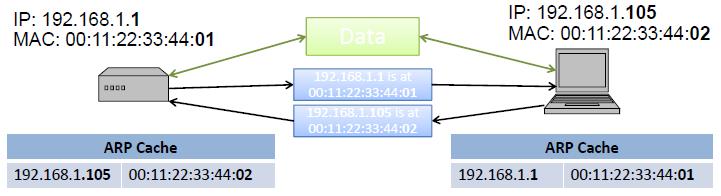
\includegraphics[height=5cm, width=10cm, keepaspectratio]{Immagini/reti/ARP_Caches.png}}
	\caption{ARP Caches\label{fig:ARP_Caches}} 	
\end{figure}
La tabella ARP contiene le corrispondenze tra gli indirizzi IP della sottorete di appartenenza e i relativi indirizzi MAC. I messaggi di request non sono tracciati e le risposte non sono verificate: il presupposto fondamentale al funzionamento del protocollo è che le macchine si fidino l'una dell'altra. Un'eventuale macchina malevola potrebbe effettuare spoofing nei confronti delle altre.
\begin{figure}[htbp]
	\centering%
	\subfigure%
	{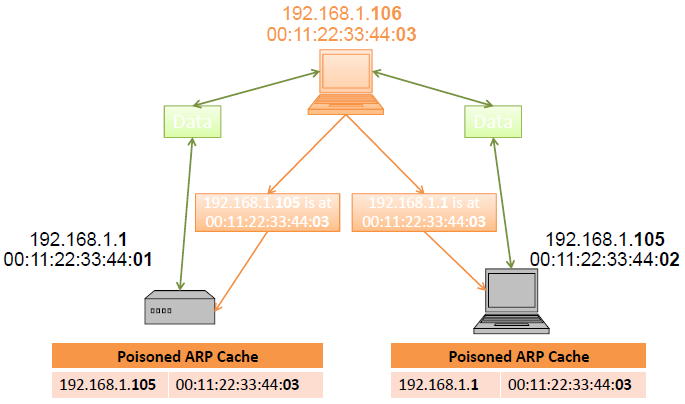
\includegraphics[height=7cm, width=10cm, keepaspectratio]{Immagini/reti/Poisoned_ARP_Caches.png}}
	\caption{Poisoned ARP Caches\label{fig:Poisoned_ARP_Caches}} 	
\end{figure}
Secondo gli standard, quasi tutte le implementazioni di ARP sono stateless, quindi la cache (\figurename~\ref{fig:ARP_Caches}) si aggiorna ogni volta che viene ricevuta una \textbf{ARP reply}, anche se non è stata inviata nessuna \textbf{request}. E' quindi facile corrompere una ARP cache semplicemente inviando reply non richiesti (\figurename~\ref{fig:Poisoned_ARP_Caches}). Si noti che utilizzare record statici risolve il problema, ma la tabella diventa ingestibile.

\section{Denial of Service Attack}
Un attacco \textbf{DoS} (\textbf{Denial of Service}) (\figurename~\ref{fig:DoS_Attack}) consiste nell'inviare un gran numero di pacchetti ad un host che fornisce un servizio, con il fine di rendere tale host (e quindi il servizio fornito) rallentato o del tutto indisponibile tramite l'esaurimento delle risorse a sua disposizione (banda, potenza di calcolo, memoria, etc.).
\begin{figure}[htbp]
	\centering%
	\subfigure%
	{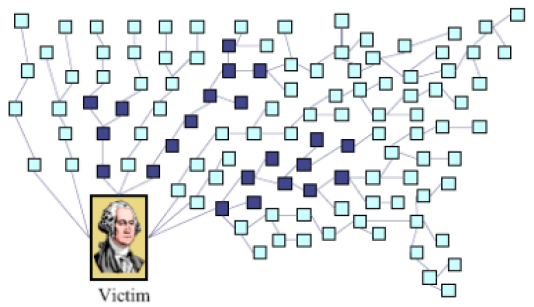
\includegraphics[height=4cm, width=12cm, keepaspectratio]{Immagini/reti/DoS_Attack.png}}
	\caption{DoS Attack\label{fig:DoS_Attack}} 	
\end{figure}
Se l'attacco parte da una sola macchina è facile da mitigare: basta infatti bloccare l'indirizzo della macchina in questione, filtrando il traffico in uscita. Per questo motivo questo tipo di attacco coinvolge solitamente una larga rete (botnet) di macchine infettate (zombie) con del software malevolo dedicato (bot). Si parla, in questo caso, di attacco DDoS (Distributed Denial of Service). Una volta creata la botnet l'organizzatore dell'attacco, al momento opportuno e controllando i bot da remoto, avvia il processo di invio pacchetti.
\newline \newline
L'attacco parte quindi dalle macchine zombie, viaggia lungo l'albero dei router di internet e arriva all'host vittima (radice dell'albero.) L'utilizzo dell'\textbf{IP source spoofing} nasconde l'attaccante e disperde il traffico che torna dall'host vittima.
\newline \newline
\paragraph{IP Traceback}
Per mitigare e prevenire questo tipo di attacchi è utile identificare gli zombie, con il fine di eliminare la botnet. Il problema dell'identificazione delle foglie dell'albero di un attacco DDoS viene detto IP Traceback. Tale problema affronta diverse difficoltà, tra cui il grande numero di router che operano in Internet, il fatto che l'attaccante possa effettuare IP Spoofing e che possa accorgersi dell'avvenimento del traceback.
\newline \newline
Alcuni approcci alla soluzione del problema sono:
\begin{itemize}
\item Filtering and tracing 
\item Messaging 
\item Logging
\item Probabilistic marking
\end{itemize}
In particolare il probabilistic marking prevede che i router "iniettino" informazione nei bit dell'header del pacchetto, inviando informazioni di routing alla vittima e avvalendosi della ridondanza per mitigare l'effetto dei pacchetti persi. Questo approccio ha diversi benefici:
\begin{itemize}
\item Non viene generato traffico addizionale
\item I router non devono memorizzare informazione
\item La dimensione dei pacchetti non cresce
\item Può essere effettuato online o offline
\end{itemize}
Altre contromisure per questo tipo di attacco sono ovviamente l'utilizzo della ridondanza e del load balancing e l'utilizzo di content provider cloud-based che regolano la capacità di fornitura dell'host in base alla quantità di richieste che riceve.

\subsection{SYN Flood}
Il SYN Flood è tipicamente un attacco DOS che si avvale delle caratteristiche del protocollo TCP, in particolare del \textbf{Three-Way handshake}. Il protocollo TCP è infatti \textbf{Connection-Oriented}, e prevede uno scambio di tre messaggi:
\begin{enumerate}
\item il client richiede la connessione al server inviandogli una richiesta rappresentata da un messaggio SYN
\item il server comunica la disponibilità inviando un messaggio SYN-ACK, e aspetta il terzo messaggio di conferma
\item il client invia un messaggio ACK per confermare la connessione
\end{enumerate}
Se il server alloca le risorse per la connessione prima della ricezione dell'ACK (eventualmente aspettando un determinato tempo) l'attacco può essere sferrato: l'attaccante crea un grande numero di messaggi SYN facendo Spoofing dell'indirizzo del mittente. Il server alloca un gran numero di risorse e risponde con dei messaggi SYN/ACK, ai quali non riceverà mai risposta. Una volta esaurite le risorse comincerà a rifiutare connessione: vi è una negazione del servizio. 
\newline \newline
Si tratta di un attacco ben noto, che non è generalmente efficace contro le reti moderne. Funziona se un server alloca delle risorse dopo aver ricevuto un SYN, ma prima di aver ricevuto un messaggio ACK. 
\newline \newline
Nel caso contrario il server dovrebbe tuttavia memorizzare lo stato della richiesta, utilizzando comunque delle risorse. Anche se l'attaccante ha bisogno di utilizzare un numero molto più grande di messaggi, l'attacco può ancora avvenire. Tra le contromisure esiste il sistema SYN cookies (disponibile su Linux o Solaris). Questa difesa usa il sequence number del pacchetto SYN-ACK per mandare un cookie al client e quindi riconoscere se quel client ha già mandato dei SYN in quella sessione, senza dover memorizzare nessuna informazione sul server. In questo modo il server non deve in alcun modo memorizzare l'arrivo dei SYN e lo stato delle richieste.

\subsection{Optimistic ACK attack}
L'attacco denominato optimistic ACK attack sfrutta il controllo di congestione del protocollo TCP. L'attaccante comincia ad inviare ACKs per segmenti di dati non ancora ricevuti, facendo credere al server che sia disponibile una grande quantità di banda, inducendolo ad aumentare la congestion window. Ciò può portare alla saturazione della banda disponile per il server, rendendo il servizio di fatto non disponile. Questo tipo di attacco può essere esteso anche a server multipli, rendendo una porzione della rete non raggiungibile dal traffico legittimo. Ad oggi non sono disponibili rimedi efficaci contro questi attacchi.
